%----------------------------------------------------------------------------------------
%	SECTION 1.1
%----------------------------------------------------------------------------------------

\section{Compact Spaces.}

\begin{definition}
    A collection $\Ac=\{A_{\alpha}\}$ of subsets of a topological space $X$ is said to be a  \textbf{cover}, or a
    \textbf{covering} of $X$ if  $\bigcup{A}=X$. We call $\{A\}$ an \textbf{open cover} if each $A$
    is open in  $X$. If  $\{A'\}$ is a subcollection of $\Ac$ that also covers $X$, we call
    $\{A'\}$ a \textbf{subcover} of $X$.
\end{definition}

\begin{definition}
    We call a topological space $X$ \textbf{compact} if for every open cover of $X$, there is a
    finite subcover of $X$.
\end{definition}

\begin{example}
    \begin{enumerate}[label=(\arabic*)]
        \item     $\R$ is not compact. Consider the following cover of  $\R$:
            \begin{equation*}
                \Ac=\{(n,n+2):n \in \Z\}
            \end{equation*}
            however, there is no finite subcollection of $\Ac$ that is a subcover of  $\R$.

        \item The subspace $X=\{0\} \cup \{\frac{1}{n}: n \in \Z\}$ of $\R$ is compact. Let  $\Ac$
            be a cover of  $X$. There is a  $U \in \Ac$ with  $0 \in U$ and $U$ contains all but
            finitely many of the points  $ \frac{1}{n}$. Now choose for each $\frac{1}{n} \in
            \com{X}{U}$ an element of $\Ac$ $A_{n}$ containing it. Then for all $n$,  $\{A_n\}$ is
            finite and covers $X$.

        \item If  $X$ is a finite topological space, then it is compact, since every open cover of
            $X$ is finite.

        \item The interval  $(0,1]$ is not compact. The open cover $\Ac=\{(\frac{1}{n}, 1]: n \in
            \Z^+\}$ contains no finite subcollection of $\Ac$ that covers  $(0,1]$. Likewise,
            $(0,1)$ is not compact by the same argument. However, $[0,1]$ is compact.
    \end{enumerate}
\end{example} 

\begin{lemma}\label{3.4.1}
    Let $Y$ be a subspace of a topological space  $X$.  $Y$ is compact if and only if every open
    cover of  $Y$, by open sets of  $X$ has a finite subcover of $Y$.
\end{lemma}
\begin{proof}
    Suppose $Y$ is compact and let  $\{A_\alpha\}$ be a cover of $Y$ with  $A_\alpha$ open in  $X$
    for all  $\alpha$. Since  $\{A_\alpha\}$ covers $Y$, so does the collection  $\{A_\alpha \cap
    Y\}$, where $A_\alpha \cap Y$ is open in  $Y$ for all  $\alpha$. Since  $Y$ is compact, choose
    the finite subcollection  $\{A_i \cap Y\}_{i=1}^{n}$ to be a finite subcover of $Y$; i.e.
    $\{A_i \cap Y\}_{i=1}^{n} \subseteq \{A_\alpha\}$.

    Conversely, suppose that for every cover $\{A_\alpha\}$, open in  $X$, of  $Y$ that
    $\{A_\alpha\}$ contains a finite subcover of $Y$. Choose  $A_\alpha'=A_\alpha \cap Y$ for all
    $\alpha$; then $\{A_\alpha'\}$ is an open cover of $Y$. 
    By hypthesis, there is a finite subcover $\{A_i\}_{i=1}^n$, and by our assignment, we
    get that $\{A_i'\}_{i=1}^n \subseteq \{A_\alpha'\}$ is also a finite subcover of $Y$. Therefore
     $Y$ is compact as a subspace of  $X$.
\end{proof}

\begin{theorem}\label{3.4.2}
    Every closed subspace of a compact space is compact.
\end{theorem}
\begin{proof}
    Let $Y$ be a closed subspace of a compact space $X$. Let $\{A_\alpha\}$ be an open cover of $Y$
    with  $A_\alpha$ open in  $X$ for all  $\alpha$. Consider  $\{B_\alpha\}=\{A_\alpha\} \cup
    \com{X}{Y}$. Since $\{A_\alpha\}$ covers $Y$,  $\{B_\alpha\}$ covers $X$. Now take some finite
    subcollection  $\{B_i\}_{i=1}^n$. If it contains $\com{X}{Y}$, then just consider
    $\com{\{B_i\}}{(\com{X}{Y})}$. Then this collection is a finite subcover of $Y$.
\end{proof}

\begin{theorem}\label{3.4.3}
    Every compact subspace of a Hausdorff space is closed.
\end{theorem}
\begin{proof}
    Let $Y$ be a compact subsapce of a Hausdorff space  $X$. Choose  $x_0 \in \com{X}{Y}$ and for
    each $y \in Y$ choose disjoint neighborhoods  $U_y$ and  $V_y$ of  $ x_0$ and $y$ respectively.
    The collection  $\{V_y\}$ covers $Y$ by open sets in  $X$, hence there is a finite subcover, by
    theorem \ref {3.4.2}, $\{V_{y_n}\}$ of $Y$. Take  $V=\bigcup_{i=1}^n{V_{y_i}}$ to be open in
$X$, and take  $U=\bigcap_{i=1}^n{U_{y_i}}$ also open in $X$. Then  $Y \subseteq V$ and  $V \cap
U=\emptyset$; for take $z \in V$,  $z \in V_{y_i}$ for some $1 \leq i \leq n$. Hence  $z \notin
U_{y_i}$, so $z \notin U$. Then  $U$ is a neighborhood of  $X$, disjoint from  $Y$, making
$\com{X}{Y}$ open in $X$. Therefore  $Y$ is closed in  $X$.
\end{proof}

\begin{figure}[h] 
    \centering
    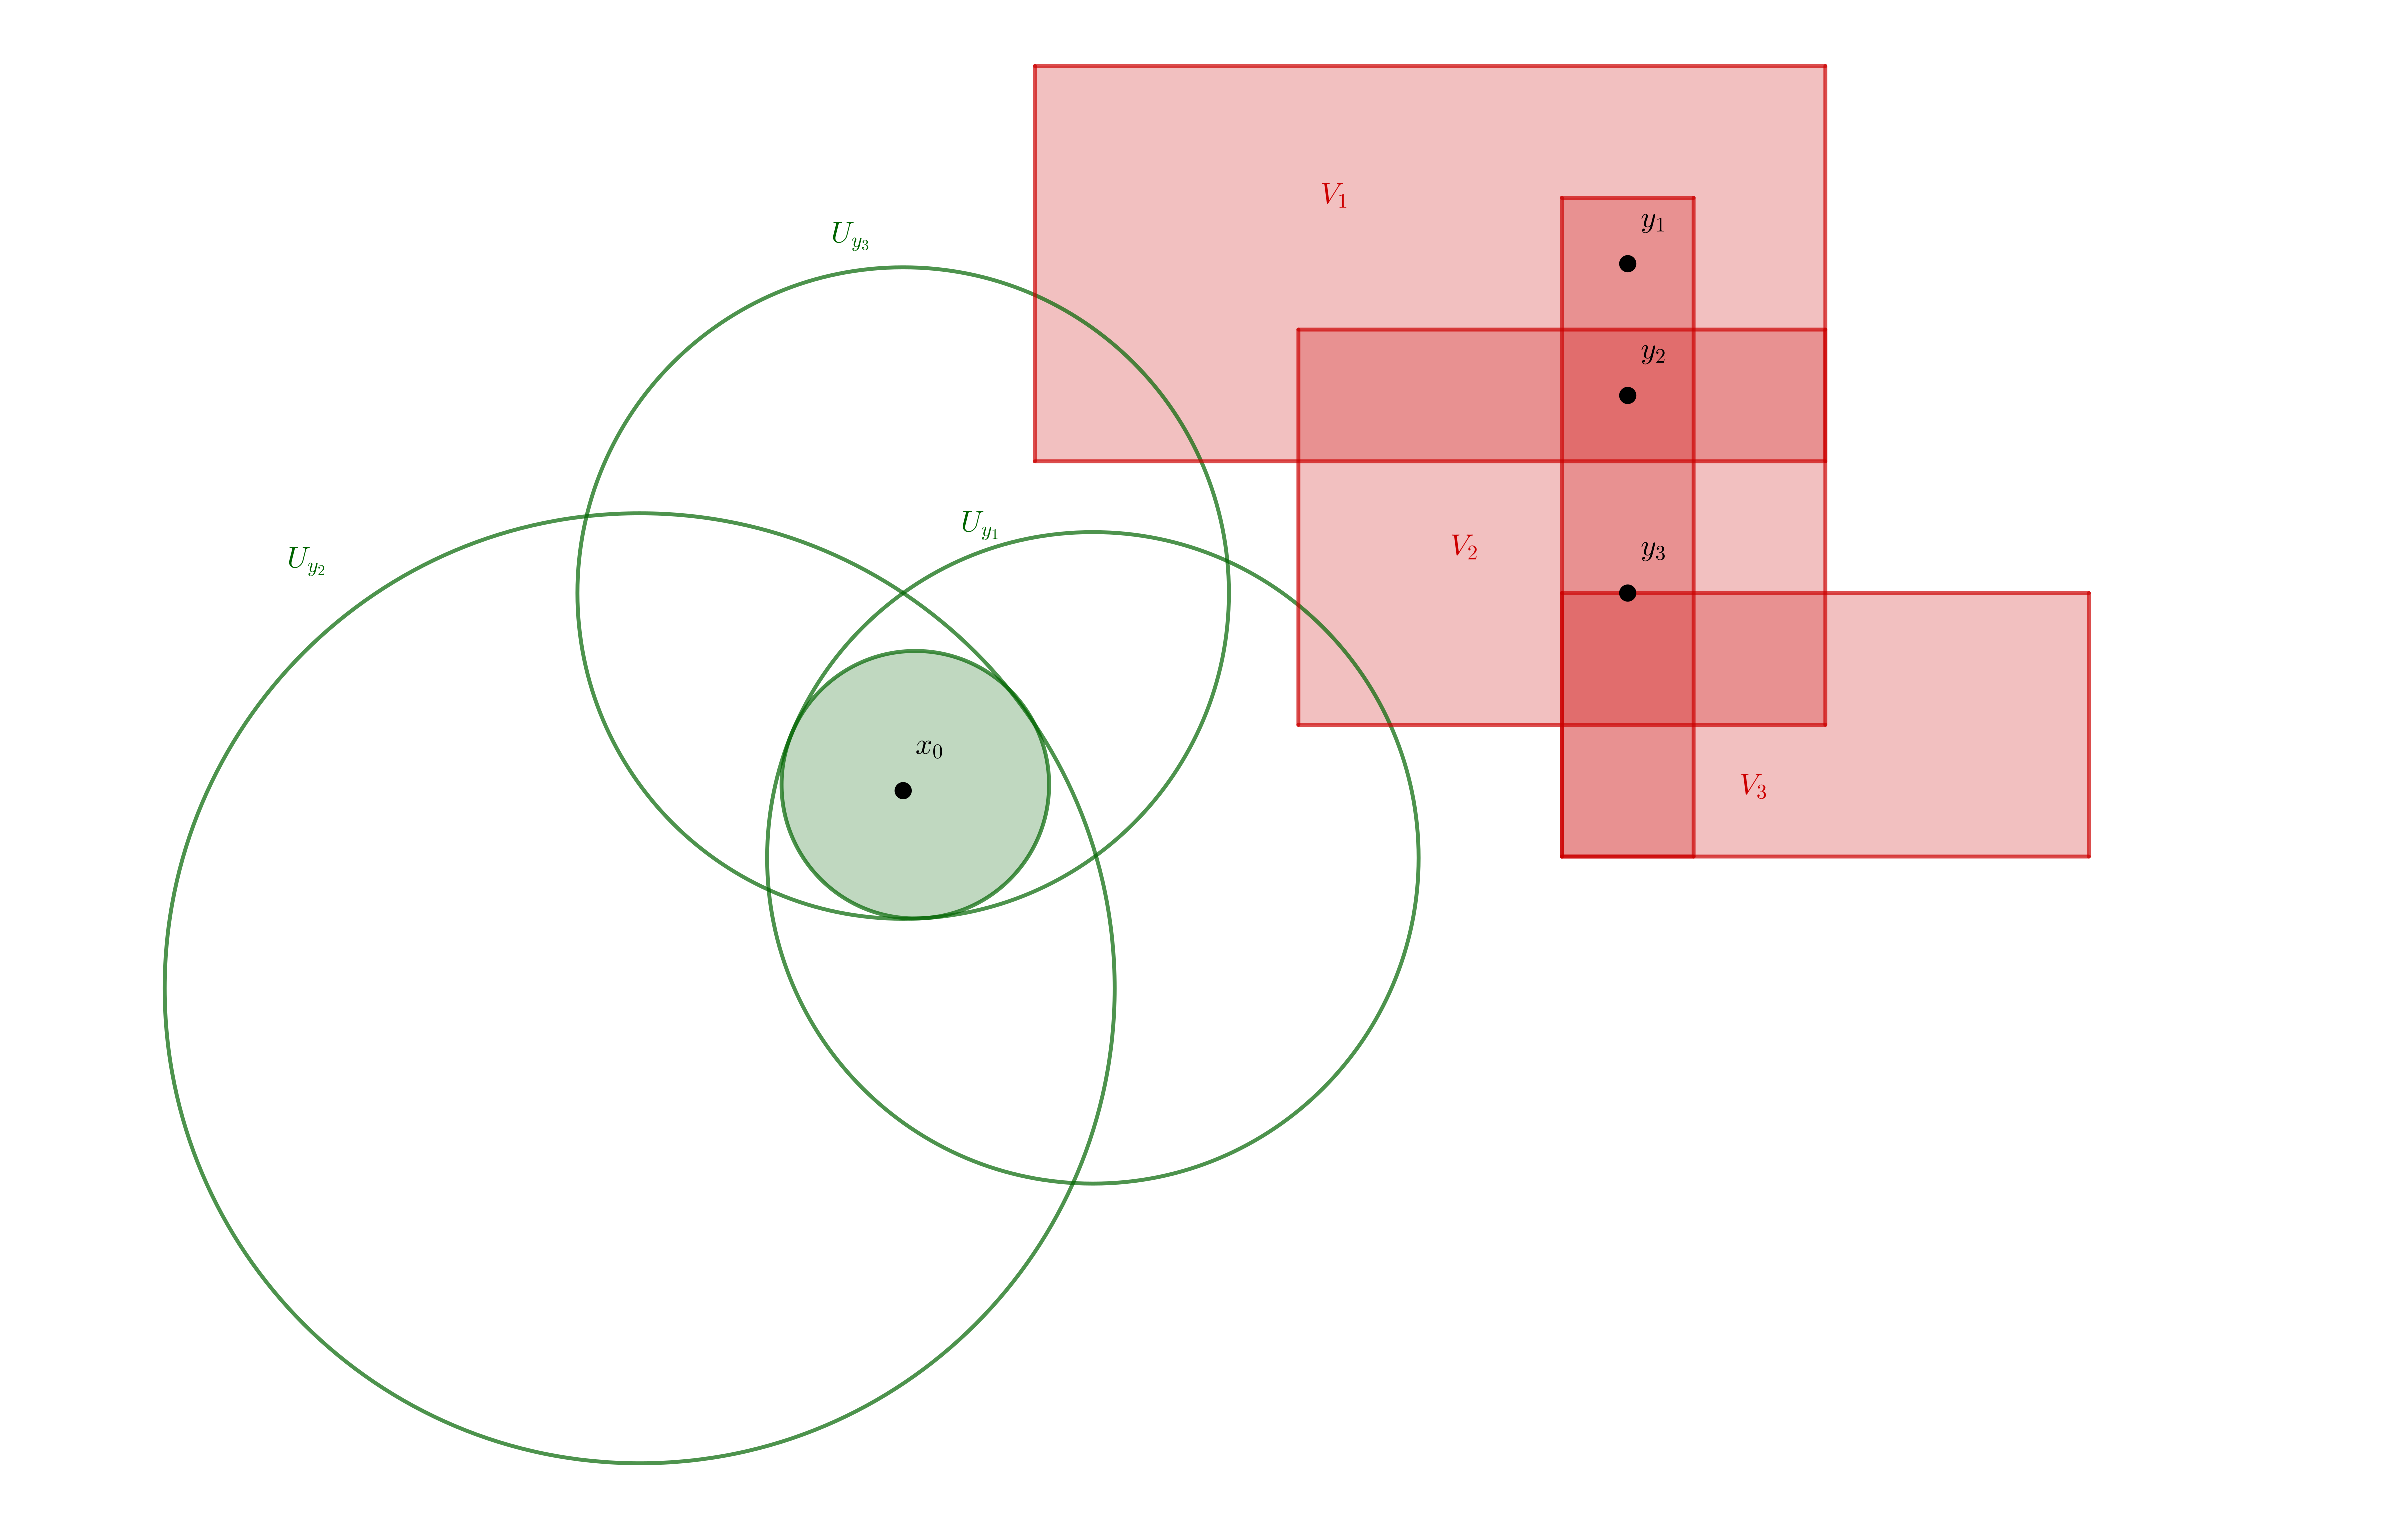
\includegraphics[scale=0.2]{Figures/Chapter3/compactHausdorff1.eps}
    \caption{}
    \label{fig_3.1}
\end{figure}

\begin{corollary}
    If $Y$ is a compact subspace of a Hausdorff space $X$, and  $ x_0 \in \com{X}{Y}$, then there
    exists opensets $U$ and  $V$ in  $X$ with  $ x_0 \in U$ and $Y \subseteq V$, respectively.
\end{corollary}
